\documentclass[12pt]{extarticle}
%\usepackage[papersize={1200px,675px},rmargin=35px,lmargin=15px,tmargin=30px,bmargin=65px]{geometry} % Twitter
\usepackage[papersize={1200px,400px},rmargin=0px,lmargin=0px,tmargin=5px,bmargin=5px]{geometry} % Secondary teaser
\usepackage{customdice}
\usepackage{rotating}


% https://latexcolor.com/
\definecolor{beaublue}{rgb}{0.74, 0.83, 0.9} % bg
\definecolor{mediumjunglegreen}{rgb}{0.11, 0.21, 0.18} % text

\definecolor{cerulean}{rgb}{0.0, 0.48, 0.65}
\definecolor{bubbles}{rgb}{0.91, 1.0, 1.0}
\definecolor{moonstoneblue}{rgb}{0.45, 0.66, 0.76}
\definecolor{golden}{rgb}{1.0, 0.84, 0.0}
\definecolor{metallicgold}{rgb}{0.83, 0.69, 0.22}

\definecolor{byzantium}{rgb}{0.44, 0.16, 0.39}
\definecolor{darkbyzantium}{rgb}{0.36, 0.22, 0.33}
\definecolor{carnationpink}{rgb}{1.0, 0.65, 0.79}


\definecolor{lavenderblue}{rgb}{0.8, 0.8, 1.0}
\definecolor{halayaube}{rgb}{0.4, 0.22, 0.33}
\definecolor{lightgoldenrodyellow}{rgb}{0.98, 0.98, 0.82}

\definecolor{lightskyblue}{rgb}{0.53, 0.81, 0.98}
\definecolor{mahogany}{rgb}{0.75, 0.25, 0.0}

\definecolor{maize}{rgb}{0.98, 0.93, 0.37}
\definecolor{limegreen}{rgb}{0.2, 0.8, 0.2}

\definecolor{mauvelous}{rgb}{0.94, 0.6, 0.67}
\definecolor{oldlavender}{rgb}{0.47, 0.41, 0.47}

\definecolor{olive}{rgb}{0.5, 0.5, 0.0}
\definecolor{olivedrab7}{rgb}{0.24, 0.2, 0.12}

\definecolor{orangepeel}{rgb}{1.0, 0.62, 0.0}
\definecolor{otterbrown}{rgb}{0.4, 0.26, 0.13}

\definecolor{midnightblue}{rgb}{0.1, 0.1, 0.44}

\definecolor{mediumturquoise}{rgb}{0.28, 0.82, 0.8}

\definecolor{mintgreen}{rgb}{0.6, 1.0, 0.6}
\definecolor{lincolngreen}{rgb}{0.11, 0.35, 0.02}

\definecolor{lightyellow}{rgb}{1.0, 1.0, 0.88}
\definecolor{mistyrose}{rgb}{1.0, 0.89, 0.88}
\definecolor{mordantred19}{rgb}{0.68, 0.05, 0.0}

\definecolor{naplesyellow}{rgb}{0.98, 0.85, 0.37}
\definecolor{oceanboatblue}{rgb}{0.0, 0.47, 0.75}

\definecolor{outerspace}{rgb}{0.25, 0.29, 0.3}
\definecolor{neonfuchsia}{rgb}{1.0, 0.25, 0.39}
\definecolor{paleaqua}{rgb}{0.74, 0.83, 0.9}

\definecolor{paleblue}{rgb}{0.69, 0.93, 0.93}
\definecolor{palechestnut}{rgb}{0.87, 0.68, 0.69}
\definecolor{palesilver}{rgb}{0.79, 0.75, 0.73}
\definecolor{pansypurple}{rgb}{0.47, 0.09, 0.29}
\definecolor{phthalogreen}{rgb}{0.07, 0.21, 0.14}
\definecolor{pistachio}{rgb}{0.58, 0.77, 0.45}
\definecolor{plum(traditional)}{rgb}{0.56, 0.27, 0.52}
\definecolor{riflegreen}{rgb}{0.25, 0.28, 0.2}
\definecolor{sandstorm}{rgb}{0.93, 0.84, 0.25}

\definecolor{whitesmoke}{rgb}{0.96, 0.96, 0.96}
\definecolor{yaleblue}{rgb}{0.06, 0.3, 0.57}

\definecolor{xanadu}{rgb}{0.45, 0.53, 0.47}
\definecolor{lightpastelpurple}{rgb}{0.69, 0.61, 0.85}
\definecolor{champagne}{rgb}{0.97, 0.91, 0.81}

\definecolor{beaublue}{rgb}{0.74, 0.83, 0.9}
\definecolor{cerulean}{rgb}{0.0, 0.48, 0.65}
\definecolor{citrine}{rgb}{0.89, 0.82, 0.04}
\newcommand{\gap}{\hspace{0.5ex}}

\begin{document}
\pagenumbering{gobble}
\nopagecolor
\Huge
\setdicefacesize{6}

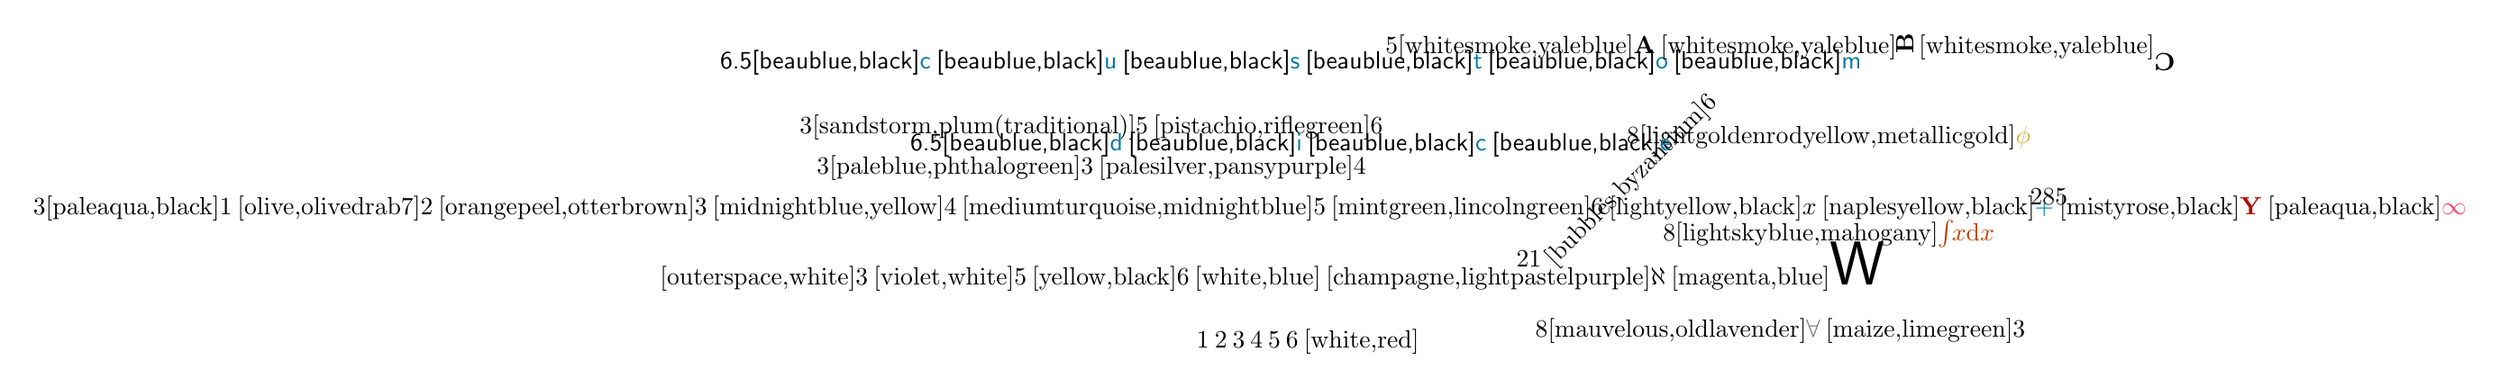
\begin{tikzpicture}[scale=2]

    \node at (1ex,-1ex) {\dice{1}\gap\dice{2}\gap\dice{3}\gap\dice{4}\gap\dice{5}\gap\dice{6}\gap\bigdotdice[white,red]};
    \node at (-0.65ex,2.5ex) {\dice[outerspace,white]{3}\gap\dice[violet,white]{5}\gap\dice[yellow,black]{6}\gap\bigdotdice[white,blue]\gap\textdice[champagne,lightpastelpurple]{\(\aleph\)}\gap\textdicebot[magenta,blue]{\Huge \sffamily W}};
    \node at (-1.7ex,5.2ex) {\setdicefacesize{3}\dice[paleaqua,black]{1}\gap\dice[olive,olivedrab7]{2}\gap\dice[orangepeel,otterbrown]{3}\gap\dice[midnightblue,yellow]{4}\gap\dice[mediumturquoise,midnightblue]{5}\gap\dice[mintgreen,lincolngreen]{6}\gap\textdice[lightyellow,black]{\(x\)}\gap\textdice[naplesyellow,black]{\color{oceanboatblue}\(+\)}\gap\textdice[mistyrose,black]{\color{mordantred19}\textbf{Y}}\gap\textdice[paleaqua,black]{\color{neonfuchsia}\(\infty\)}};
    
    \node at (-9.08ex,7.1ex) {\setdicefacesize{3}\dice[paleblue,phthalogreen]{3}\gap\dice[palesilver,pansypurple]{4}};
    \node at (-9.08ex,9ex) {\setdicefacesize{3}\dice[sandstorm,plum(traditional)]{5}\gap\dice[pistachio,riflegreen]{6}};
    
    
    \node at (35.5ex,5.75ex) {\setdicefacesize{28}\dice{5}};
    \node at (15.5ex,6.5ex) {\setdicefacesize{21}\rotatebox{45}{\dice[bubbles,byzantium]{6}}};
    
    
    \node at (25.25ex,4ex) {\setdicefacesize{8}\textdice[lightskyblue,mahogany]{\color{mahogany}\normalsize\(\int\hspace{-1mm}x \mathrm{d}x\)}};
    \node at (23ex,-0.5ex) {\setdicefacesize{8}\textdice[mauvelous,oldlavender]{\color{oldlavender}\(\forall\)}\gap\dice[maize,limegreen]{3}};
    
    \node at (25.25ex,8.5ex) {\setdicefacesize{8}\textdice[lightgoldenrodyellow,metallicgold]{\color{metallicgold}\(\phi\)}};
    
    \node at (0.2ex,12ex) {\sffamily\setdicefacesize{6.5}\textdice[beaublue,black]{\color{cerulean}c}\gap\textdice[beaublue,black]{\color{cerulean}u}\gap\textdice[beaublue,black]{\color{cerulean}s}\gap\textdice[beaublue,black]{\color{cerulean}t}\gap\textdice[beaublue,black]{\color{cerulean}o}\gap\textdice[beaublue,black]{\color{cerulean}m}};
    \node at (0.2ex,8.2ex) {\sffamily\setdicefacesize{6.5}\textdice[beaublue,black]{\color{cerulean}d}\gap\textdice[beaublue,black]{\color{cerulean}i}\gap\textdice[beaublue,black]{\color{cerulean}c}\gap\textdice[beaublue,black]{\color{cerulean}e}};
    
    \node at (23ex,12.5ex) {\setdicefacesize{5}\textdice[whitesmoke,yaleblue]{\textbf{A}}\gap\textdice[whitesmoke,yaleblue]{\rotatebox{90}{\textbf{B}}}\gap\textdice[whitesmoke,yaleblue]{\rotatebox{180}{\textbf{C}}}};
    
\end{tikzpicture}



\end{document}